\documentclass[12pt]{article}
\usepackage[utf8]{inputenc}
\usepackage{graphicx}
\usepackage{amsmath}
\usepackage{hyperref}
\usepackage{geometry}
\geometry{margin=1in}

\title{Interim Progress Report}
\author{Priyangika Pitawala}
\date{\today}

\begin{document}

\maketitle

\section*{Project Title}
Image Analysis and Percent Crystallinity Quantification

\section{Introduction}
This project involves creating a Python-based tool that processes polarized optical microscope (POM) images of a semicrystalline
thiol-ene photopolymer system, and analyzes the percent crystallinity. It will also attempt to find a correlation between the percent
crystallinity and the thermal and mechanical properties obtained from experimental data.

\section{Objectives}
\begin{itemize}
    \item To preprocess the POM images to enhance the contrast between crystalline and amorphous regions, and to reduce noise.
    \item To define the features that characterize crystallinity and develop an algorithm to distinguish between crystalline and amorphous regions.
    \item To calculate the percent crystallinity of each image and aggregate the results of multiple images using statistical methods.
    \item To analyze the relationships between the percent crystallinity and the polymer properties.
    \item To use data visualization tools to display the results.
    
\end{itemize}

\section{Methodology}

\subsection{Key steps and dependencies}

Key steps include:
\begin{itemize}
    \item data loading of polarized optical microscope (POM) images.
    \item preprocessing to prepare for image segmentation.
    \item segmentation using edge-based techniques and watershed algorithm.
    \item crystallinity feature extraction.
    \item percent crystallinity quantification.
    \item regression and visualization.
    
\end{itemize}

All steps are separated into modules and can be found inside the `src/` subfolder.\\

The dependencies are numpy, matplotlib, opencv-python, scikit-image, scipy, and pandas. A comprehensive list can be found in `requirements.txt` file inside the `docs/` subfolder.

\subsection{Preprocessing requirements}

\begin{itemize}
    \item Grayscale conversion as image segmentation doesn't require color channels.
    \item Noise reduction using Gaussian blur and further filtering.
    \item Masking of known foreground and background.
    \item Edge detection using Canny operators.
    \item Gradient magnitude thresholding to highlight crystal boundaries.
    \item Morphological operations to clean the binary image.
    \item Computation of segmentation markers.
\end{itemize}

\subsection{Computational strategies}
\begin{itemize}
    \item Separate modules for handling the key steps.
    \item Interactive exploration, real-time parameter tuning, and segmentation validation using Jupyter notebooks.
    \item Vectorization of the image processing steps using NumPy and/or SciPy.
\end{itemize}

\subsection{Efficiency and optimization strategies}
\begin{itemize}
    \item Version control by intermittently committing the progress to  GitHub, especially prior to tuning parameters to optimize segemntation.
    \item Image downsampling by removing unnecassary information such as color channels. 
\end{itemize}

\section{Project Progress Assessment}

I have worked on initial research, data preparation, gradient computation, edge-based segmentation, watershed algorithm, and feature extraction steps.
These tasks were supposed to be completed by Week 11 as detailed in my previous Gantt chart. 
However, the feature extraction step has shown that the image segmentation (and therefore, the preprocessing) step must be optimized further to improve the accuracy. 
Nevertheless, the current model is providing an acceptable result and framework to qualitatively compare all my POM images.\\

The updated work schedule is as follows:
\begin{itemize}
    \item Week 12: Refine image segmentation further; complete extracting the crystallinity features; calculate percent crystallinity.
    \item Week 13: Regression analysis and model interpretation.
    \item Week 14: Finalize analysis and data visualization. 
\end{itemize}

No scope adjustment is needed if the segmentation can be refined before the end of Week 12. 
However, if more time is needed to achieve that, the scope will be adjusted to qualitative rank each image for 
percent crystallinity based on the model performance, instead of calculating a quantitative number.\\

The updated gantt chart is as follows:

\begin{figure}[h!]
    \centering
    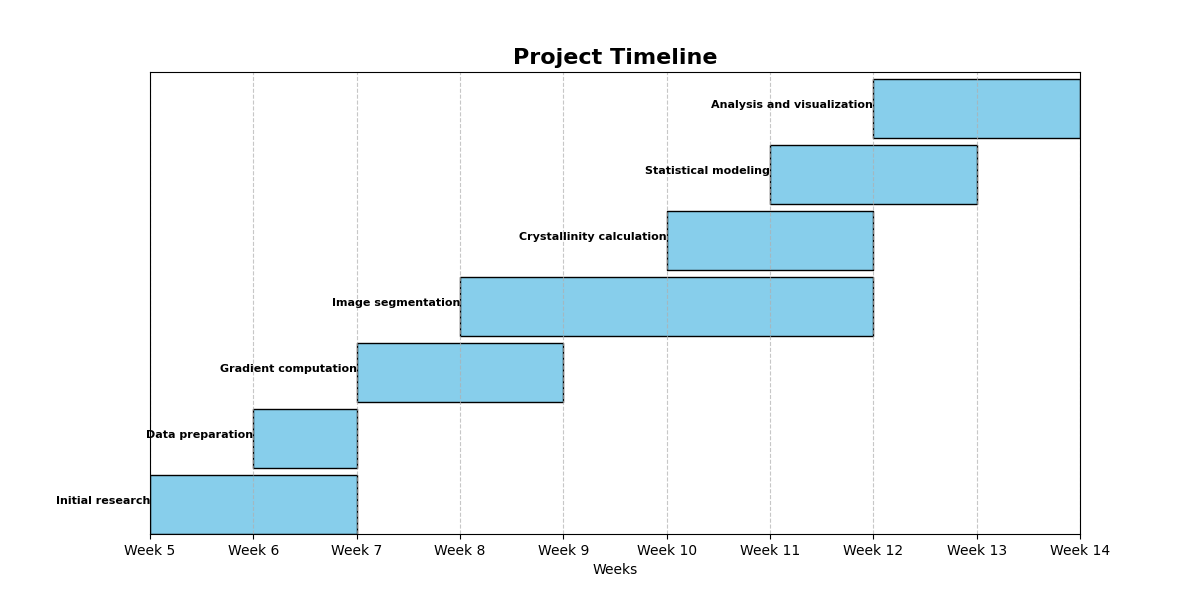
\includegraphics[width=\textwidth]{gantt_chart.png}
    \caption{Updated Gantt chart showing planned project timeline.}
\end{figure}

\section{References}

\begin{enumerate}
    \item Gonzalez, R. C.; Woods, R. E. \textit{Digital Image Processing}, 4th ed.; Pearson: Boston, MA, 2018.
    \item OpenAI. \textit{ChatGPT}; https://chat.openai.com (accessed March 30, 2025).
\end{enumerate}

\end{document}
